        \documentclass[11pt,oneside,a4paper]{scrartcl}
\renewcommand{\familydefault}{\sfdefault}
\usepackage{amsmath}
\usepackage{helvet}
\usepackage{titleref}
\usepackage[utf8x]{inputenc}
\usepackage[english]{babel}
\usepackage{fancyhdr}
\usepackage{graphicx,caption}
\usepackage{subfig,amsmath}
\usepackage{setspace}
\usepackage{longtable}
\usepackage{wasysym}
\usepackage{geometry}
\usepackage{gensymb}
\usepackage{color}
\usepackage{colortbl}
\geometry{a4paper,left=2cm,top=1cm, top=1.5cm, bottom=3.5cm}
\makeatletter
\renewcommand\paragraph{\@startsection{paragraph}{4}{\z@}%
  {-3.25ex\@plus -1ex \@minus -.2ex}%
  {1.5ex \@plus .2ex}%
  {\raggedsection\normalfont\sectfont\size@paragraph}%
}
\makeatother
%\renewcommand\thesection{\arabic{section}}

\begin{document}

\vspace*{1cm}
\pagestyle{fancy}
\fancyhf{}
%Kopfzeile rechts bzw. au�en
\fancyhead[RO]{Florian Kraemer}
%Kopfzeile links bzw. innen
\fancyhead[LO]{\today}
%Linie oben
\renewcommand{\headrulewidth}{0.5pt}
%Linie unten
\renewcommand{\footrulewidth}{0.5pt}
\addtolength{\headheight}{30pt}



\vspace*{2cm}
\begin{center}
\vspace*{0.5cm}
\textbf{\Huge Sensordata}
\vspace*{2cm}
\\ An Android-application to read, store and display compressed sensordata\\
\end{center}

\vspace*{3cm}

\begin{center}
\textbf{\LARGE} Florian Kraemer \\
\end{center}

\newpage % Ende vom Text

\tableofcontents

\newpage

\setcounter{page}{1}
\pagestyle{fancy}
\fancyhf{}
%Kopfzeile rechts bzw. aussen
\fancyhead[RO]{Florian Kraemer}
%Kopfzeile links bzw. innen
\fancyhead[LO]{\textbf{\large Sensordata}}
%Linie oben
\renewcommand{\headrulewidth}{0.5pt}
%Fu�zeile rechts bzw. au�en
\fancyfoot[C]{\thepage}
%Linie unten
\renewcommand{\footrulewidth}{0.5pt}
%\addtolength{\headheight}{10pt}

\onehalfspacing
\setcounter{section}{0}

\section{Objectives}
Smartphones offer a wide range of use. We want to use their fair processing power, storage capacity and attached sensors to allow easy handling of sensor networks. Thus the task is to develop an Android application that is capable of receiving data from sensor nodes via the telecommunication network, processing, storing and displaying them in a significant way. Furthermore managing the metadata of each node on a phone will make it user-friendly to find nodes, alter positions in an existing sensor-network or install new nodes. Challenges are to keep the application as modular as possible, to allow changes to the supported sensor-network, such as the number of sensors, the number of platforms or switching between compression algorithms. The smartphone is not intended for storing the data forever. Taking their hardware capabilities into consideration and having smartphones in the field requires to backup the data regularly. But connecting to a web-service would also allow for using for example a tablet for displaying data. It is also important to make the application usable on different devices featuring different screen sizes and processing power or telecomunication features.
The following graph shows the general build-up of the system.


\begin{center}
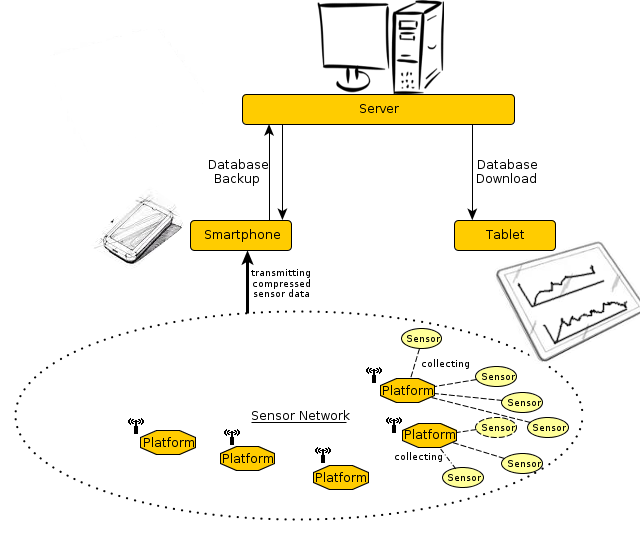
\includegraphics[scale=0.6]{picture/general_buildup.png}\\
\textit{Graph of the whole system}
\end{center}

\subsection{The supported sensor-platform}
The current release of the application supports a platform with four sensors, each having two subsensors, one for moisture- and one for temperature measurements. An additional sensor is used to collect battery data. The data is then compressed with a Huffman-Code, a method developed by Rachel Cardell-Olivier, and transmitted in a SMS-message.


TODO insert footnote

\section{Architecture}
\subsection{Overview}
The application features several activities for the different types of user-interactions. \\
Then there is an underlying service, that handles the background data-processing. It reads, decompresses and stores the sensordata from the phone's SMS-inbox. It also handles which numbers are interpreted to be platforms and to which platform in the database they should correspond Besides this it also provides the connection between the activities and the database and saves the users preferences to a file.

\subsection{Data model}
An existing data model  FOOTNOTE was reduced to fit the specifications of a smartphone application. This reduces the amount of choices the user has to make in order to operate and keeps the complexity to a certain level. It also makes the database as lightweight as possible. The measurement entity-type features no dedicated id, but instead the timestamp and subsensor id are used as a unique primary key.

\begin{center}
\begin{tabular}{|c|c|}
\hline \textbf{ Entity-type} &  \textbf{Attributes} \\ 
\hline platform & id,description,period,latitude,longitude,mobile number \\ 
\hline sensor & id,latitude offset, longitude offset, elevation offset, platform id \\ 
\hline subsensor & id, phenomena id, sensor id \\ 
\hline measurement & timestamp, measurement, subsensor id \\ 
\hline phenomena & id, description, unit, maximum, minimum \\ 
\hline 
\end{tabular} 
\end{center}


\section{Implemention}
\subsection{Activities}
The current release uses just six activities. This is possible due to recycling of two of them: Depending on the intent they are started with, the choose-a-platform-activity and the change-a-platform-activity react differently. This makes sense, since very similar actions like altering and inserting new metadata for a platform require the same layout and it prevents duplicate code. It is also possible to use an object-orientated approach here, but for the little differences keeping a low number of classes and therefore the overview had a higher priority.
The following graph shows the behaviour of the different activities, the arrows indicate from where the different activities are triggered and the dotted ones to which activity the user will be send upon pressing the phone's back-button.

\begin{center}
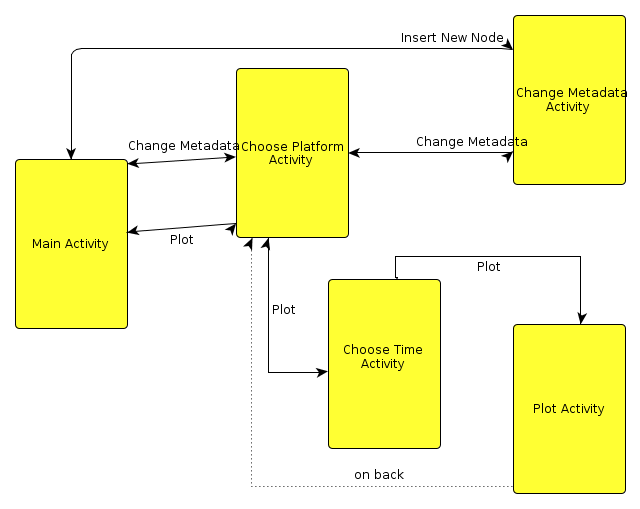
\includegraphics[scale=0.6]{picture/sensordata_activities.png}\\
\textit{Graph of activities}
\end{center}

\subsubsection{Main}
This activity is launched on startup and used to offer accessibility to the different features of the application.

\subsubsection{Choose Platform}
This activity is used twice. One time on the path to choose the metadata and another time to plot data. The platforms are displayed using two different item-layouts, since it is only of interest to see which  platform is the receiving one, when the user has the option to change this in the following activity. 

\subsubsection{Change Platform}
In this activity all the metadata can be viewed and except from the mobile number and id changed. This activity is also used to add new platforms and mobile numbers, in which case the user will be prompted to enter the number on startup. The phone's GPS-sensor is used to receive the current coordinates, which are then displayed and saved in microdegrees.

\subsubsection{Choose Period}
This activity offers at this time five different options to choose from and will then set the period to be displayed in the plot. The first two simply set static time periods, going back one day or one week from the time of execution.
The other three query the database to set a period that goes back one day or one week from the last entry or shows all entries for this platform.

\subsubsection{Plot data}
Here two plots are arranged to visualize the preselected data. Special about this one is, that it will resize the plots according to the individual screen size. This offers multi-device support and is even important when turning the device to view the data in the landscape view. It is payed attention to, that even in small screen sizes there is enough space to scroll the view and for bigger sizes to keep everything in one window to avoid unnecessary scrolling. Also the range of maximum shown time differs depending on the screen size to provide as much data as possible while still keeping the graphs readable. Smaller devices may just see 12hours of data, while a tablet might be able to view three days at a time.
This of course is also basically depending on the periods with which the data is collected and the current preferences are not dynamic, but rely on a period of about 30minutes. TODO

\subsubsection{Database}
In this activity a connection with a ftp-server can be etablished to send or retrieve the database-file. The apache-commons-net library is used for this. The network related actions are executed in AsyncTasks, so the main thread is not stressed by it or blocked in the worst case. To show the user of what is happening in the background there are different dialogs deployed to show the working progress and explain what went wrong in case of an exception. This actually is a quite complex situation, with files being read and written from internal and external storage and also using an internet connection at the same time. The possible exceptions are passed by throw-clauses to suggest to the user in the end what went wrong.
Do ensure the integrity of the local database at least to a certain level, the file is first saved on the external storage and once that is completed successfully this new database is copied and then 
replaces the old local one. Always copying the whole database file provides definitely just a temporary solution, due to the unflexibility and dangers to the file-integrity concerning bigger database sizes.
If using a webservice at this point there would also be a need to eveluate the incoming data in order if and where to insert it into the database. Whether there were new messages received is indicated by a boolean set in DataService.


INSERT FOOTNOTE

\subsection{Data service}
A service in Android can be used applications to handle (long-running) operations in background. Activities can bind to it and then call its public methods. Different to activities it does not provide a user-interface, thus only toasts and notifications can be used to inform about its state. The data service actually provides a notification once it has decompressed a new message.
The main duties of the dataService are to handle messages, pass on the funtionality of the database and save the settings of the application for the next start.

\subsubsection{Handling incoming messages}
The service is continiously checking the inbox for new messages and if necessary, decompresses them, deletes them from the inbox and saves the processed data into the database. A flag, that there is an update for the server, will also be set and saved to a file and the period can be set as a constant.
The data-model offers one physical platform to be deployed at several coordinates. This might result in multiple virtual platforms with the same mobile number. The strategy to identify the corresponding platform, while just knowing the mobile number from the text message is to keep an internal list for the currently receiving platforms. This is implemented so that one mobile number can just link to one platform id and new inserted ones will be automatically set up to be the receiving authority.
If the number is not linked in this list, the database will be prompted for the mobile number. It might return a platform and in case of finding multiple it will return the one to which data was added most recently. This is then just a good guess, but the user is expected to set up the platforms properly before they send the messages. In the worst case of everything being unsuccessfull so far a new platform will be created with empty metadata fields. 

The decompressing is logged to the SD-card's application folder into the smsdata-file. This involves logging the timestamp, when it was received, the timestamp contained in the message and the status of the decoding including possible exception-messages.

\subsubsection{Binding - Offering methods}
The service uses the easiest of several complex and unconvenient ways offered by Android to provide the link to activities, thus non-static objects. Every binding activity must provide a MyConnection (\textit{implements ServiceConnection}), which then saves the actual DataService-object through a Binder. This shall not be illustrated any more here, but from then on the public DataService-methods can be used easily. Note that binding and unbinding must be done pairwise in onStart/onStop to not provoke Exceptions of leaked connections.

\subsubsection{Saving the current state}
Here the shared preferences are another, cleaner way to go, but saving the current preferences to .txt-files was a side product of the logging and proved to be efficient and reliable.
Basically there are a few lines written, that contain: The flag, whether there is an update for the server, tuples of mobile numbers and the currently receiving platforms id in the database and finally a list of numbers that are taking into consideration when scanning the inbox.


\subsection{Database}
Android supports SQLite databases by default and the direct interactions with it are done in the DatabaseControl-class, which should itself just be prompted by the DataService-class ( see \textit{\ref{sec:database_safety} \titleref{sec:database_safety}} ). The nested subclass DBHelper handles the creating, openening and copying of the database. All Strings are set as public constants here to allow easy access and changes. The ``\_{}id '' is specifically named like this, since for example the CursorAdapter used in the ChoosePlatform-Activity for a ListView requires it to work properly. An essential detail is the ON UPDATE CASCADE property, that keeps the relations of tables intact although the foreign keys are altered. This is not used in paticular right now, but should be considered important when communicating with another database, since this might involve updating foreign keys. The ON DELETE CASCADE is used to delete all dependent table rows in the database. Thus the user can delete a complete platform including all its measurements in the Change-Platform-activity. This makes sense, since measurements without a linked platform will not be selectable to be plotted anymore and therefore are dead data. Note that executing the sql-command ``PRAGMA foreign\_{}keys=ON;'' after creating the tables is substantial for the ON DELETE CASCADE to work.

The database is quite unflexible right now, meaning it is tailored for the current build-up with nine incoming data streams. Also the phenomenas are created hardcoded right now upon startup.


\subsection{Plotting}
To visualize the data the library androidplot is used. It offers a wide range of preferences, but a rather sparse API. The biggest challenge here is to find the limits for displaying as much data as possible while still making it wel-readable and handable for the user. Thus it might just be a well-sized extract from the chosen data.
Since the plots are implementing a touch functionality, the shown ranges are limitted with maximum and minimum values, so one can not get lost in the depth of the graph. 
To make the touch experience a bit smoother, a thread was implemented, that slows the scrolling and zooming exponentially down after the touch gesture, instead of stopping immediately.
To not allow the view to be scrolled on smaller screen sizes a custom scrollview was implemented, that allows to block scrolling the view while gestures are made on the plots.

INSERT FOOTNOTE

\subsection{Thread safety}
The Android platform comes with a mannerism, that necessitates special handling at times. The most important constraint is that changes to the views can only be done from the UI-thread. When using multithreading thus attention must be paid to this. The Android API provides the AsyncTask, its doInBackground-method offers background processing, while its onPostExecute-method is executed in the UI-thread and can therefore be used to meet this challenge.
In the current release CountdownLatches are used to prevent from problems upon binding to the underlying service. This process takes some time and when put for example in the OnStart-method of an activity, it is not determined to be executed at the expected time.

\subsubsection{Accessing the database}\label{sec:database_safety}
The advantage of using one service for all actions, that involve the database, is a good overview. It is openend and closed securely just in the start and destroy methods and the resource can be locked for a single binder-thread on demand. Actually this not often necessary, since just the getSms-thread, that checks for new sms periodically and writes data to the database, and a user-invoked thread to read from it could interact at one time. This does not endanger the data-integrity, but having different numbers of timestamps and measurements will provoke an exception in the plot-activity.
What might do this, is a user trying to change the metadata while measurements are added. TODO
Also while overwriting the existing database with a downloaded one, the getsms-thread should not try to write. TODO
\section{Debugging}\label{sec:Debugging}
The Android-plugin for Eclipse makes it fairly easy to create a virtual device or debug the application directly on a phone connected by wire to the PC . The phone must have the USB debugging options activated, which can be done in the settings. The convenient eclipse debugger tools can then be used with the usual features like break-points and reading variables during runtime. The Android tool LogCat does also display Exceptions and other runtime output of the application. Depending on the phone this might have to be activated in very individual ways, possibly through hidden settings.

One is likely to encounter odd errors, when trying to debug or just run parts of the package through a standard java main-method: This is solved by correcting the run configurations for the java application, since the bootstrap entries in the classpath are set to the Android library, instead of the current JRE and JUnit libraries.


\section{Testing}
\subsection{High-level and on-device}
Since the application can be started on devices during development as described in \textit{\ref{sec:Debugging} \titleref{sec:Debugging}}, it is very convenient to test the correct behaviour of the application just on the device. This includes using different devices to ensure for example correct presentation on different screen sizes or hardware compability.

\subsection{database benchmarks}
TODO: 10years,10platforms, period:30min... too mouch

\section{Risks}
Upon reinstallation, which must for example be done, when changing the development PC \underline{all} data of the application is lost. This involves database backups, the preference file and log file on the SD-card.


\section{Future Tasks}
These would involve:

\begin{itemize}
\item
Setting up a RestFul-Webservice, that collects the (multiple) phones data centrally in a global database. This would probably involve .php-scripts for the actual webservice interactions and packing the data in .xml or .json-files to transfer it. On the Android side there are helper classes for JSON.
A strategy must be developed to merge the two or multiple databases, since several phones are not bound to unique keys any more. 

\item
Change the phone side to interact dynamically with the server. It has to backup the local data, when it got updated. Querying the global database it should receive only a certain amount of data or just a certain period back in time. The user could be prompted in a new activity or another possibility is to query and buffer the data while the user scrolls the plot.

\item
The plots could compare several platforms for the same or different time. It would probably make sense to show average values instead of four line charts for each platform.

\end{itemize}

\section{links}
sqlite sheets
android api
vogella
mybringback.com


\end{document}
